\chapter{Challenge III}

\section{Outline}
\begin{enumerate}
   \item A user can launch an instance of a compiler C
   \item When launching the instance, the user specifies the name of the
   source file
   \item When the compilation is over, the user specifies the name of the
   file to store the output code
   \item The compiler updates a file log with the accounting information
   so that users pay for using the compiler
\end{enumerate}

\begin{table}[htbp]
   \centering
   \begin{tabular}{c|c|c|c|c|}
      & Compiler & \texttt{input} file & \texttt{output} file &\texttt{log} file\\
      \hline
      User & \texttt{execute} & \texttt{read} & \texttt{write} &\\
      \hline
      Compiler & & & & \texttt{write}\\
      \hline
      \textit{Instance} & & \texttt{read} & \texttt{write} & \texttt{write}\\
   \end{tabular}
   \caption{Outline schema}
   \label{tab:ch3_outline}
\end{table}
\begin{center}
   \textit{What happens if the user transmits as the name of the output file the one of the logfile?}
\end{center}

\section{In-class discussion}

The key issue according to prof. Baiardi is that the article asserts that ACLs and capabilities are not equivalent, because ACLs do not allow to prevent the attack while capabilities can.

Solve the problem using ACLs.
\underline{"There is a \textit{very very very} simple solution."}\nl

A simple idea is to not grant the \texttt{write} right to the compiler but the \texttt{append} right,
leading the compiler to simply append to the log file both the output of the compilation and the actual log.
This is not a proper solution, but still is a nice countermeasure.

\begin{table}[htbp]
   \centering
   \begin{tabular}{c|c|c|c|c|}
      & Compiler & \texttt{input} file & \texttt{output} file &\texttt{log} file\\
      \hline
      User & \texttt{execute} & \texttt{read} & \texttt{write} &\\
      \hline
      Compiler & & & & \texttt{append}\\
      \hline
      \textit{Instance} & & \texttt{read} & \texttt{write} & \texttt{append}\\
   \end{tabular}
   \caption{Outline schema}
   \label{tab:ch3_inclass}
\end{table}


\newpage

\section{Proposed Ideas}
I gave a quick look at \href{https://waterken.sourceforge.net/aclsdont/current.pdf}{this \textit{"ACLs don't"} article}, it may be the one cited by the professor when presenting the challenge.

\begin{paracol}{2}
   The article proposes a sligthly different ACM than the one outlined in class \ref{tab:ch3_outline}.
   \begin{table}[htbp]
      \centering
      \begin{tabular}{c|c|c|c|c|}
         & Compiler & \texttt{input} file & \texttt{output} file &\texttt{log} file\\
         \hline
         User & \texttt{execute} & \texttt{read} & \texttt{write} &\\
         \hline
         Compiler & & \texttt{read} & \texttt{write} & \texttt{write}\\
         \hline
         \textit{Instance} & & \texttt{read} & \texttt{write} & \texttt{write}\\
      \end{tabular}
      \caption{Article's ACM}
      \label{tab:ch3_articleACM}
   \end{table}
\switchcolumn

\begin{figure}[htbp]
   \centering
   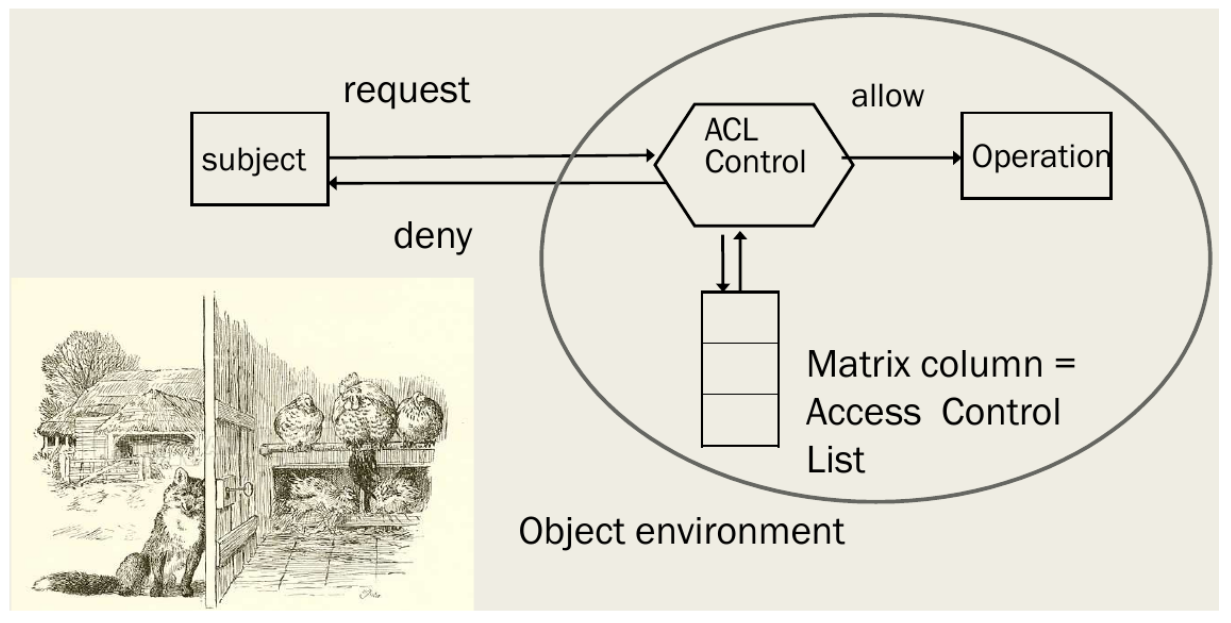
\includegraphics[width=0.9\columnwidth]{images/ACL_schema.png}
   \caption{ACL schema}
   \label{fig:ACL_schema2}
\end{figure}
\end{paracol}

Recalling the ACL schema \ref{fig:ACL_schema2} presented in class, article's ACM \ref{tab:ch3_articleACM} makes sense:
since it's the compiler (i.e. \textit{subject} in Fig. \ref{fig:ACL_schema2}) which \textit{requests} to read the \texttt{input} file to write onto the \texttt{output} file the result of the compilation,
the lookup in the ACM will be performed on the \textit{Compiler} row, not the \textit{User}'s one.\\
To summarize the point made in the article,
the user requests to execute \texttt{compiler("input.c","a.out")}, and after such operation is granted,
it will be the \texttt{compiler} to request permission for further operations, i.e. reading input, writing output and, lastly, logging.\\
in case a malicious user invokes \texttt{compiler("input.c","log.json")},
when the compiler requests to write the compilation output to \texttt{"log.json"}, the operation {---}since the compiler has write right on \texttt{"log.json"}{---} is allowed,
resulting in the log file to be overwritten (\textbf{"confused deputy"} problem).\nl

I think that here lies the key issue:
if the check in the ACM is done on the User's row the compiler does \textit{not} need write access to output file and thus cannot be \textit{"confused"}.

The compiler should write the compilation result in a "working" directory that a User can only read,
and then it should be the User to request to read such compilation result and then to write it to desired output,
forcing the ACM check to be performed on the User's row, not the compiler one. 

\begin{table}[htbp]
   \centering
   \begin{tabular}{c|c|c|c|c|>{\columncolor{verylightgray}\color{gray}}c<{\color{black}}}
      & Compiler & \texttt{input} file & \texttt{output} file &\texttt{log} file & working \texttt{dir}\\
      \hline
      User & \texttt{execute} & \texttt{read} & \texttt{write} & & \texttt{read}\\
      \hline
      Compiler & \texttt{read} & & & \texttt{append} & \texttt{write}\\
      \hline
      \textit{Instance} & & \texttt{read} & \texttt{write} & \texttt{append} &\texttt{write}\\
   \end{tabular}
   \caption{Proposed ACM}
   \label{tab:ch3_sol2}
\end{table}

\section{Alternative Solution - Decomposition}

A different approach, which instead requires more consistent changes in the software architecture, would imply decomposing the compiler in two components/modules:
\begin{enumerate}
   \item \textit{Compiler} producing the output file, and writing log records in a temporary \texttt{tmp} file\footnote{distinct from output file}.
   \note{A pipe, a socket or a generic temporary file the writeable by \textit{Compiler} and readable by \textit{Logger}}
   \item \textit{Logger} which receives (and validates) info to be logged from the \textit{Compiler}
\end{enumerate}
In this way we can define the security policy according to the \textbf{Least Privilege} principle, negating the \texttt{log} file \texttt{write} right to the \textit{compiler} and granting \texttt{append} only to the \textit{logger},
resulting in the following ACM:

\begin{table}[htbp]
   \centering
   \begin{tabular}{c|c|c|c|c|c|>{\columncolor{verylightgray}\color{gray}}c<{\color{black}}}
      & Compiler & \texttt{input} file & \texttt{output} file & \texttt{tmp} file &\texttt{log} file & working \texttt{dir}\\
      \hline
      User & \texttt{execute} & & & & &\\
      \hline
      Compiler & & \texttt{read} & \texttt{write} & \texttt{write} & & \texttt{write}\\
      \hline
      Logger & & & & \texttt{read} &\texttt{append} &\\
      \hline
      \textit{Instance} & & \texttt{read} & \texttt{write} & \texttt{write} & \texttt{append} &\texttt{write}\\
   \end{tabular}
   \caption{Decomposition ACM}
   \label{tab:ch3_sol2.1}
\end{table}